% Created 2021-05-10 Mon 19:34
% Intended LaTeX compiler: pdflatex
\documentclass[11pt]{article}
\usepackage[utf8]{inputenc}
\usepackage[T1]{fontenc}
\usepackage{graphicx}
\usepackage{grffile}
\usepackage{longtable}
\usepackage{wrapfig}
\usepackage{rotating}
\usepackage[normalem]{ulem}
\usepackage{amsmath}
\usepackage{textcomp}
\usepackage{amssymb}
\usepackage{capt-of}
\usepackage{hyperref}
\usepackage{awesomebox}
\usepackage{booktabs}
\usepackage{placeins}
\usepackage{siunitx}
\usepackage{minted}
\usepackage[capitalise]{cleveref}
\newcommand{\gv}[1]{\ensuremath{\mbox{\boldmath$ #1 $}}}
\newcommand{\bv}[1]{\ensuremath{\boldsymbol{#1}}}
\newcommand{\norm}[1]{\left\lVert#1\right\rVert}
\newcommand{\imag}[1]{\mathrm{Im} \left[ #1 \right]}
\newcommand{\order}[1]{\mathcal O \left( #1 \right)}
\newcommand{\abs}[1]{\left\lvert#1\right\rvert}
\newcommand{\RN}[1]{\textup{\uppercase\expandafter{\romannumeral#1}}}
\usepackage{setspace}
\singlespacing
\setminted[powershell]{fontsize=\footnotesize}
\usepackage[lmargin=1.0in, rmargin=1.0in, tmargin=1.0in, bmargin=1.0in]{geometry}
\newcommand{\cpp}{\texttt{C++} }
\newcommand{\mse}{\textrm{MSE}}
\newcommand{\pde}{\ensuremath{\mathcal{P}}}
\newcommand{\Ltwo}[1]{\ensuremath{\mathcal{L}_2\left[#1\right]}}
\definecolor{violet}{RGB}{89,99,225}
\newcommand{\newcontent}[1]{\textcolor{violet}{#1}}
\newcommand{\todo}[1]{\textcolor{red}{TODO -- #1}}
\author{CS498DL, Spring 2021}
\date{}
\title{Physics informed neural networks for problems involving nonlinear differential equations.\\\medskip
\large Project report}
\hypersetup{
 pdfauthor={CS498DL, Spring 2021},
 pdftitle={Physics informed neural networks for problems involving nonlinear differential equations.},
 pdfkeywords={},
 pdfsubject={},
 pdfcreator={Emacs 28.0.50 (Org mode 9.3.6)},
 pdflang={English}}
\begin{document}

\maketitle

\section{Team details}
\label{sec:org6c892e9}
\begin{center}
\begin{tabular}{lll}
\toprule
Name & NetID & Department\\
\midrule
Bhosale, Yashraj & bhosale2@illinois.edu & Mechanical Science and Engineering\\
Chan, Fan Kiat & fchan5@illinois.edu & Mechanical Science and Engineering\\
Parthasarathy, Tejaswin & tp5@illinois.edu & Mechanical Science and Engineering\\
\bottomrule
\end{tabular}
\end{center}

\section{Updates}
\label{sec:org69da6f5}
For ease in readability and grading, updates to the report (from the first
checkpoint) and new results \newcontent{are marked in violet, like this}
\newcontent{sentence}. Finally, all code used to generate results in the report can be
found \href{https://github.com/fankiat/CS498DL-project}{in this repository (click here)}.

\section{Problem summary}
\label{sec:org6a1aaa6}
\newcontent{
We implement and investigate Physics-Informed Neural Networks, a deep-learning approach for solving non-linear
partial differential equations. We demonstrate PINNs' ability to solve
equations of increasing complexity, from linear, 1D problems to nonlinear, 2D
problems, based only on the problem description and without the need of fine
numerical discretization or problem-specific algorithms.
}

\begin{figure}[htbp]
\centering
\includegraphics[width=1.0\textwidth]{images/CS498DL_cropped.eps}
\caption{\label{fig:cs498_poisson_results}Solution of a Poisson equation generated by Physics-Informed Neural Networks within the shape \emph{CS498DL}. Each alphanumerical character is prescribed with a unique boundary condition resulting in varied, rich solutions seen in the interior.}
\end{figure}

\newpage

\section{Introduction and background}
\label{sec:orgfff21aa}
\newcontent{
In this report, we implement and investigate Physics-Informed Neural Networks
(PINNs), a deep-learning approach for generating numerical solutions
of non-linear partial differential equations (nPDEs). We are motivated by utilizing
the recent rapid advances in data-driven techniques in machine learning (ML)
and deep learning (DL) to solve nPDEs, as an alternative to conventional
numerical approaches which are both mathematically and computationally
intensive. Rather PINNs take minimal effort to set up, doesn't require domain
knowledge (of PDEs) and is hence ideal as a black-box solver which once trained,
can rapidly produce solutions to arbitrary numerical PDEs. In the rest of this
section, we introduce the reader to PDEs and conventional numerical approaches to
solve them, which in turn motivates the need for alternative methods such as PINNs.
 }

\subsection{Partial differential equations}
\label{sec:orgccb257c}
Partial differential equations (PDE) are ubiquitous in science and
engineering. Mathematically, a PDE imposes relations between various partial
derivatives of a multi-variable function within a system of interest. These
relations capture fundamental physical laws governing a system (e.g.
Newton's equations of motion) such as those associated with sound, heat,
diffusion, electrostatics, electrodynamics, fluid dynamics, elasticity,
general relativity, and quantum mechanics \cite{wiki:pde}.

Such PDEs are broadly categorized as initial-value problems (IVPs) and boundary-value problems
(BVPs). Roughly speaking, IVPs involve \emph{evolution} of a function as time
progresses, from some initial condition, such as a trajectory function of a ball
dropped from a height. In contrast, BVPs involve finding a static solution \emph{satisfying
constraints} on given boundaries, such as finding the temperature distribution
of a room with a constant temperature heater embedded in one wall.

Many PDEs of practical interest (such as those governing fluid-dynamics)
demonstrate behavior of both IVPs and BVPs. The solution to such PDEs are
crucial in revealing physics to enable new applications (such as
targeted therapeutic drug-delivery within our fluidic blood vessels, for
curing diseases) or optimizing design of existing applications (such as
improving models of aero-planes for efficient transport) or for predictive
forecasting (such as predicting weather). Unfortunately, these PDEs are
usually non-linear (i.e. they belong to the category of non-linear partial differential equations, nPDEs),
and we do not \emph{apriori} know their closed-form mathematical solutions.

\subsection{Numerical solution to partial differential equations}
\label{sec:org2de1e66}

To solve these nPDEs then, we turn to numerical solutions. The traditional
approach here is to numerically \emph{discretize} the nPDE over a large grid of
floating-point variables in space-time. We then numerically solve, via
computer simulations, the PDE locally at every point in the grid.
Finally, we reconstruct the PDE solution using these local discretizations.
This field has a rich tradition over the past \textasciitilde{}70 years \cite{quarteroni2008numerical} and multiple
techniques for efficiently solving IVPs and BVPs exist. As a result it has
been quite successful in achieving its goals, especially with the recent advent of
modern, parallel supercomputers which provide capabilities for accelerated simulations.

Despite its varied successes, this field is not without challenges. To
achieve satisfactory results, the mesh spacing of the grid needs to be
smaller than the smallest feature size of the target solutions. This often is
not feasible because of the curse of dimensionality: achieving \(10 \times\) higher
resolution usually requires \(10^4 \times\) more compute, because the
grid must be scaled in four dimensions---three spatial and one temporal.
Then, to satisfactorily solve these numerical equations we need faster and larger simulations. But in
recent years, Moore's (predictive) law has been slowing \cite{waldrop2016more} and we are
approaching the limits of Dennard scaling \cite{esmaeilzadeh2011dark}, which
restricts design of general-purpose microprocessors, which consequently
stifles simulation speeds even with parallelism.
\newcontent{
Another challenge relates to the wide variety of numerical algorithms needed.
In fact, different PDEs require vastly different numerical strategies to
ensure physical fidelity of \emph{discrete} solutions in the computer. Developing
the theory for such strategies is usually mathematically cumbersome and
time intensive, especially when new PDEs need to be modeled.
}

\subsection{PINNs}
\label{sec:orgaeac313}
An alternative approach to solving PDEs numerically, aiming to partially
offset the aforementioned challenges, involves utilizing data-driven
techniques popularized by the advent of machine learning
(ML) \cite{bar2019learning}. Such approaches efficiently utilize data sampled
from systems of interest to learn the representation of underlying nPDEs. They
also take advantage of recent algorithmic breakthroughs in ML along with fast hardware
(such as TPUs) and software (such as frameworks) optimized for these applications.

An attractive candidate among these approaches is the Physics-Informed Neural
Network (PINN). These are models trained to solve self-supervised learning
tasks adhering to given laws of physics \cite{raissi2019physics} described
by general nPDEs. As such, only the initial and boundary data are needed to
recover solutions to arbitrary nPDEs---the network generates incorrect
solutions while training and uses these solutions to learn, and
converge to the correct result.
\newcontent{
Additionally, they are easy to setup and efficiently run on modern hardware architectures,
thanks to automatic differentiation and abstracted kernel (GPU) implementations in
recent, popular deep learning software frameworks \cite{paszke2019pytorch}.
These features make it an attractive candidate for use as a black-box
multi-physics solver across engineering domains.
}
Finally, recent works on PINN have shown promise in
\emph{instantly} predicting results for IVP governed by nPDEs across
scientific domains, for example in
incompressible fluid dynamics \cite{jin2020nsfnets,raissi2020hidden}, reaction--diffusion systems in
computational chemistry \cite{raissi2019physics}, and the propagation of nonlinear
waves in quantum mechanics. PINNs can also generate solutions for
BVPs in complex domains, such as those found in continuum
solid mechanics.

\subsection{Deliverables}
\label{sec:org79d77c0}
\newcontent{
Having motivated the need for ML approaches such as PINNs for solving PDEs,
}
\begin{enumerate}
\item We propose to implement the algorithm for such PINNs and validate it
against a time-independent BVPs with known (numerical) solutions (such as
Laplace or Poisson equation), as well as against time-dependent IVPs (such
as the Burger’s equation).
\item Finally, if time permits, we will extend the method for solving problems
of higher complexity. In particular, we are interested in solving problems
in the field of fluid mechanics \cite{jin2020nsfnets,raissi2020hidden}, with
focus on problems where no known analytical solutions are available
and direct numerical simulation approaches are computationally expensive.
\end{enumerate}

\section{Results}
\label{sec:orgb45679f}
We demonstrate our results by considering PINN solutions to increasingly
complex PDEs in a step-by-step fashion. Particularly, we start by
describing the implementation of such PINNs. Then we consider a sequence of
PINN solutions to 1D BVPs (Poisson, Helmholtz), and build up our PINN machinery
which we utilize to generate solutions to more complex spatio-temporal nPDEs
(Burgers, 2D Poisson).

\subsection{Implementation details}
\label{sec:orgbba7158}
Here we consider BVPs as parametrized PDEs of the form
\[ \mathcal{P}[u ; \lambda] = 0, x \in [0, 1] \]
where \(x\) denotes the solution domain, \(u : x \mapsto \mathbb{R}\)
denotes the latent solution embedded in
our deep network, and \(\pde[\cdot, \lambda]\) is the operator defining the PDE,
parametrized by our PINN weights (and biases) \(\lambda\). These
parameters \(\lambda\) are learnt over a self-supervised training process
where we only provide the PDE to be satisfied and boundary data.
We now describe our network architecture, loss functions and training protocols used to implement PINNs.

\subsubsection{Network architecture}
\label{sec:org7c8f50e}
We design our PINNs to take input points \(x_i,~i = 1, \dots,  N_\pde\)
sampled \(\in [0, 1]\) as a vector \(\in \mathbb{R}^{N_\pde}\).The total
number of input points \(N_\pde\) is chosen based on the desired resolution. The network then
generates potential solutions
\(u_i \in \mathbb{R}^{N_\pde}\) as outputs, sampled at the same points.

Throughout this report our PINN utilizes a multi-layer perceptron, comprising of 2
hidden, fully-connected layers of 50 neurons each with a hyperbolic tangent
(\(\tanh\)) activation function. Our choice of \(\tanh\) activation is
necessary to accelerate learning by allowing back-propagation of non-zero
gradients, thus bypassing dead ReLU problems.
Other complex activation functions \cite{jagtap2020adaptive} are possible---here we
skip these to retain simplicity in our networks.

Finally, after these hidden layers, we have a fully-connected
50-neuron output layer bereft of any activation. The lack of final layer
activation is motivated by our need to capture arbitrary PDE and
boundary-value dependent scales and shifts of PDE solutions. If we
enabled a similar \(\tanh\) activation here, it puts the total network
output in the limited range [-1, 1], which curtails the representation power
of our network and consequently destroys any potential for generalization to
arbitrary PDEs. With this fixed model, we proceed to train our network.

\subsubsection{Loss function}
\label{sec:org9165bb2}
During training, we minimize the loss of sum of mean squared errors
associated with the PDE \(\pde\) and boundary data \(u_{b}\). That
is the total loss \(\mse\) is defined as
\[ \mse := \lambda_{\pde} \mse_{\pde} + \mse_{b} \]
where the \emph{PDE loss} \(\mse_{\pde}\) is defined as
\[ \mse_{\pde} :=  \Ltwo{\pde[u(x_i)]}\]
where \(\Ltwo{\cdot}\) is the discrete L2 norm defined as
\[ \Ltwo{f} := \frac{1}{N_\pde}\sum_{i=1}^{N_\pde} \abs{f(x_i)}^2 \]

The PDE loss above enforces adherence of latent solution \(u\) to \(\pde\) across
points sampled within the domain \(x_i,~i = 1, \dots,  N_\pde\). The second
loss \(\mse_{b}\) enforces adherence of \(u\) to boundary values and is called the
\emph{boundary loss}, defined as
\[ \mse_{b} :=  \frac{1}{N_b}\sum_{j=1}^{N_b} \abs{u(x^b_j) - u_b(x^b_j) }^2\]
where \(N_b\) denotes the number of boundary points and the sum here is
over all boundary points \(x^b_j,~j = 1, \dots,  N_b\).

To adjust the relative importance the network provides to conformation to
the PDE in the interior points versus the boundary points, we use the
hyper-parameter \(\lambda_{\pde}\), which we set to \(1\) in our
experiments, unless noted otherwise.

\subsubsection{Training protocol}
\label{sec:org7b1a560}
One attractive feature of PINNs for generating PDE solutions is that its training
is not data intensive. Indeed, PINNs are self-supervised and works in
sparse-data limits---it only needs the PDE structure and boundary
information! Hence, in this project, we do not train it over huge datasets,
as a result of which training time is manageable, taking only a
\newcontent{couple of minutes across all presented cases},
on both our local machines and Google Colaboratory servers.

Training for all architectures presented here is done with the Adam
optimizer \cite{kingma2014adam} with a training rate of \(2.5 \times
	10^{-3}\), for 15000 epochs,
with other parameters set to their recommended default.

Once the training is completed, we then need to test fitness of generated
solutions \(u\). For linear PDEs, we have analytical solutions \(\hat{u}\), which depends on the problem and boundary conditions, against
which we compare \(u\). This \(\hat{u}\) is specified as and when needed,
from \cref{sec:poisson} onwards. It is also sampled along the network points \(x_i,~i = 1, \dots,  N_\pde\). This allows us to define a network error \(e := \sqrt{\Ltwo{u - \hat{u}}}\), which we use to gauge solution
fitness---smaller errors are better.

In contrast, for nonlinear PDEs, we lack analytical solutions. Here we then
adopt two metrics to gauge solution fitness:
\begin{itemize}
\item We measure the residual \(\sqrt{\Ltwo{\pde[u]}}\). This indicates how well
\(u\) satisfies the PDE. Smaller residuals are better.
\item We obtain numerical solutions \(u_{h}\), using finite-differences,
against which we compare \(u\), to produce discrete error \(e_h\)
defined as \(e_h := \sqrt{\Ltwo{u - u_{h}}}\). Once again we use this discrete
error \(e_h\) to gauge solution fitness---smaller errors are better.
\end{itemize}
A fit solution is marked by small magnitudes across both these metrics.

This concludes our section on model choice and training. We now use this
model to investigate performance of
PINNs for generating solutions to PDEs of increasing complexity.

\subsection{PINN solutions of 1D Poisson equation}
\label{sec:poisson}
We start by investigating PINN solutions of simple linear PDEs with
established theoretical results against which we compare. Here, we consider
solutions \(u : x \mapsto \mathbb{R}, x \in [0, 1]\) to the 1D Poisson equation, described by
\begin{equation}
\label{eqn:poisson}
\begin{aligned}
	\pde[ u ] &:= \nabla^2 u  - f = 0 \\
	   		  &:= \frac{\partial^2 u}{\partial x^2} - f(x) = 0
\end{aligned}
\end{equation}
coupled with suitable boundary conditions. We start with the Poisson equation
as it is the workhorse
underlying virtually all scientific and engineering domains. As a more
concrete example, it is useful in heat-transfer applications such as thermal
regulation of indoor spaces. Here the Poisson \cref{eqn:poisson} governs the
distribution of temperature (modeled using \(u\)) within a room with heat
sources/sinks (modeled using \(f\)) with, say, insulated walls (modeled using
boundary conditions). Here we do not model such applications in full
complexity, rather we focus
on a toy problem capturing the essence of generating solutions to the 1D
Poisson \cref{eqn:poisson}.

In this equation, we first demonstrate our ability to account for varied boundary
conditions in our PINN architecture for a fixed function \(f\):
\[ f(x) = 10 \left(\sin(\pi x) + 2\sin(2\pi x) + 3\sin(3\pi x) + 10\sin(4\pi
   x) + 10\sin(5\pi x)\right) \]
This sinusoidal forcing is chosen for producing relatively complex
solutions with multiple bumps and troughs, despite its simplicity in description.
With this \(f(x)\) we then compare our PINN results against known
analytical solutions.
\begin{figure}[htbp]
\centering
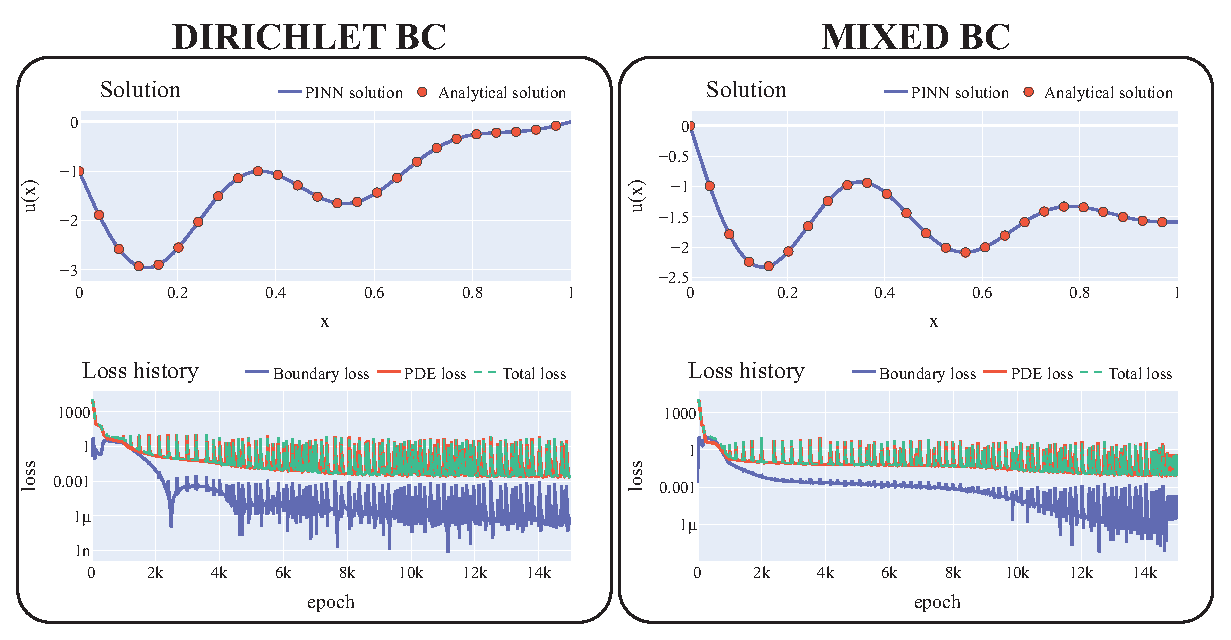
\includegraphics[width=1.0\textwidth]{images/poisson.eps}
\caption{\label{fig:poisson_results}PINN results (solution and loss histories) for the 1D Poisson equation shown for (left) Dirichlet boundary conditions and (right) mixed Dirichlet--Neumann boundary condition. The PINN solutions are depicted by solid, blue lines while scatter points represent reference analytical solutions.}
\end{figure}

\subsubsection{Dirichlet boundaries}
\label{sec:orge32ce6b}
In this regard, we first solve \cref{eqn:poisson} with Dirichlet (or) constant-value
boundary conditions
\[ u_b(0) = -1 ;\quad  u_b(1) = 0\]
For this case, our analytical solution is
\[ \hat{u}(x) = -1 + x - \frac{10}{\pi^2} \left(\sin(\pi x) + \frac{1}{2}\sin(2\pi x) + \frac{1}{3}\sin(3\pi x) + \frac{5}{8}\sin(4\pi
	x) + \frac{2}{5}\sin(5\pi x)\right) \]
We train our PINN with \(N_\pde = 100 , N_b = 2\) and recover the solutions
shown in the left column of \cref{fig:poisson_results}, along with its loss
histories. We see that our PINN
solution agrees with the analytical one,
with \(e = 4.6 \times 10^{-4}\). The loss history is dominated by \(\mse_\pde\) and steadily decreases with increasing epochs.

\subsubsection{Mixed Dirichlet--Neumann boundaries}
\label{sec:org9d68767}
Next we demonstrate solutions of \cref{eqn:poisson} with Neumann (or)
constant-slope boundary condition on the right boundary and retain Dirichlet
conditions on the left boundary.
\[ u(0)_b = 0 ;\quad \frac{\partial u_b}{\partial x}(1) = 0\]
For this case, our analytical solution is
\begin{equation}
	\begin{aligned}
	 \hat{u}(x) &= \frac{10}{\pi}\left(\cos(\pi) + \cos(2\pi) + \cos(3\pi) + \frac{5}{2}\cos(4\pi) + 2\cos(5\pi)\right)x \\
	 & - \frac{10}{\pi^2} \left(\sin(\pi x) + \frac{1}{2}\sin(2\pi x) + \frac{1}{3}\sin(3\pi x) + \frac{5}{8}\sin(4\pi
	 x) + \frac{2}{5}\sin(5\pi x)\right)
	\end{aligned}
\end{equation}
We again train our PINN with \(N_\pde = 100 , N_b = 2\) and recover the solutions
shown in the right column of \cref{fig:poisson_results}, along with its loss
histories. We see that our PINN solution agrees with the analytical one,
with \(e = 2.7 \times 10^{-4}\). The loss history is dominated by \(\mse_\pde\) and steadily decreases with increasing epochs.

\subsection{PINN solutions of 1D Helmholtz equation}
\label{sec:helmholtz}
Next, we consider solutions to more complex linear problems. Here, we
consider solutions \(u : x \mapsto \mathbb{R}, x \in [0, 1]\) to the 1D Helmholtz equation, described by
\begin{equation}
\label{eqn:helmholtz}
\begin{aligned}
	\pde[ u ] &:= \left(\nabla^2 + k^2 \right) u - f = 0 \\
	   		  &:= \frac{\partial^2 u}{\partial x^2} + k^2 u - f(x) = 0
\end{aligned}
\end{equation}
coupled with suitable boundary conditions. Here, \(k \in \mathbb{R}\)
denotes a constant wave number and introduces additional
complexity to \cref{eqn:helmholtz} when compared to \cref{eqn:poisson}. Helmholtz equations
are typical in scenarios
involving waves (for e.g. in acoustics and electromagnetic radiation) and
subsequent applications (for e.g. in noise-cancelling headphones). Here
it governs the amplitude of sound (modeled using \(u\)) within a room with noise
sources/sinks (modeled using \(f\)) with, say, perfectly sound-proof walls
(modeled using boundary conditions).

While we demonstrated our ability to handle different boundary conditions in
\cref{sec:poisson}, here we demonstrate our ability to account for arbitrary forcing
functions \(f(x)\) in our PINN architecture. We achieve this for fixed, Dirichlet
boundary conditions
\[ u_b(0) = 0;\quad  u_b(1) = 0\]

\begin{figure}[htbp]
\centering
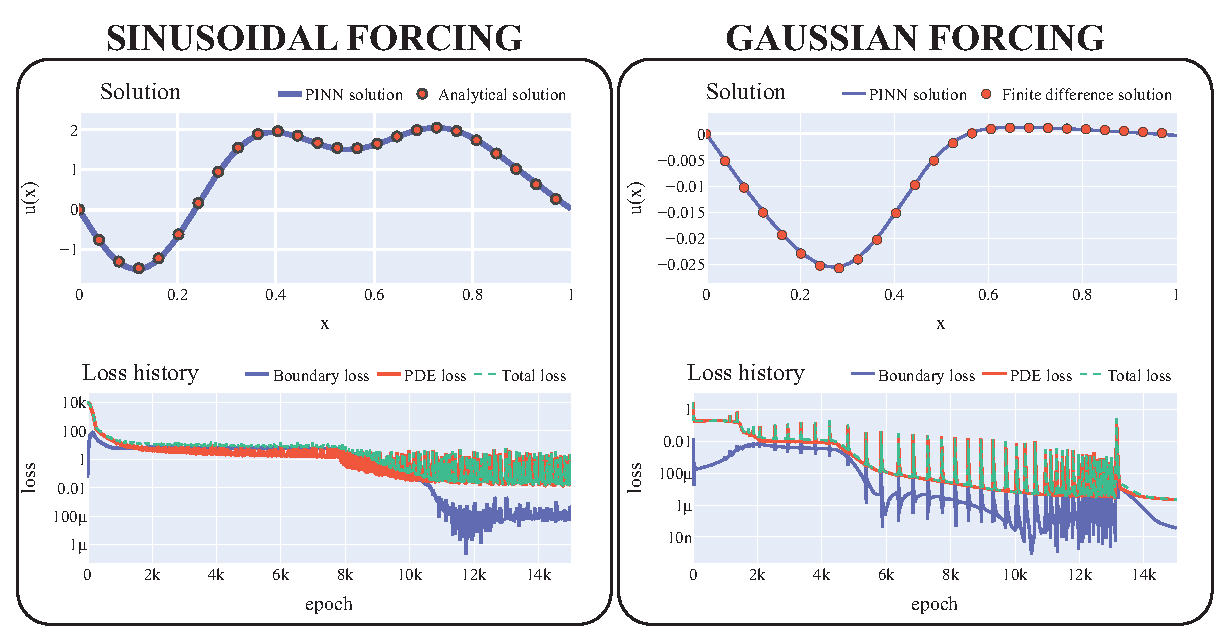
\includegraphics[width=1.0\textwidth]{images/helmholtz.eps}
\caption{\label{fig:helmholtz_results}PINN results (solution and loss histories) for the 1D Helmholtz equation shown for (left) sinusoidal forcing and (right) gaussian forcing. The PINN solutions are depicted by solid, blue lines while scatter points represent reference analytical/finite-difference solutions.}
\end{figure}
\subsubsection{Sinusoidal forcing}
\label{sec:org9d289cc}
In this regard, we first solve \cref{eqn:helmholtz} for \(k = 4\) with the
same forcing equation as in \cref{sec:poisson}, reproduced below for convenience.
\[ f(x) = 10 \left(\sin(\pi x) + 2\sin(2\pi x) + 3\sin(3\pi x) + 10\sin(4\pi
   x) + 10\sin(5\pi x)\right) \]
For this case, our analytical solution is
\begin{equation}
\begin{split}
  \hat{u}(x) = 10 &\left(\frac{1}{4^2 - \pi^2}\sin(\pi x) + \frac{2}{4^2 -
	 \left(2\pi\right)^2}\sin(2\pi x) + \frac{3}{4^2 -
   \left(3\pi\right)^2}\sin(3\pi x) \right. \\
 & \left. + \frac{10}{4^2 - \left(4\pi\right)^2} \sin(4\pi
   x) + \frac{10}{4^2 - \left(5\pi\right)^2}\sin(5\pi x) \right)
\end{split}
\end{equation}
We train our PINN with \(N_\pde = 100 , N_b = 2\) and recover the solutions
shown in the left column of \cref{fig:helmholtz_results}, along with its loss
histories. We see that our PINN solution agrees with the analytical one,
with \(e = 2 \times 10^{-2}\). Regarding training history, we see that the
loss is dominated by \(\mse_b\) at early stages of training, and later
dominated by \(\mse_\pde\). In other words, the PINN
has difficulty adjusting to boundary conditions in the first 10k epochs,
beyond which it finds the right set of solutions, marked by a decrease in
boundary loss. For the PDE loss, we observe a similar decrease around 8k
epochs but this time the behavior is comparatively less pronounced.

\subsubsection{Gaussian forcing}
\label{sec:orgc64cb81}
Next we demonstrate solutions of \cref{eqn:helmholtz} with a non-sinusoidal
forcing demonstrated below, consisting of two Gaussian bumps
\[ f(x) = \exp\left[-\left(\frac{(x - 0.3)}{0.1}\right)^2\right] -  \exp\left[-\left(\frac{(x -
   0.5)}{0.1}\right)^2\right] \]
In this case analytical solutions are not easy to obtain, so we turn to numerical
solution \({u}_h\) based on finite-differences. We again train our PINN with
\(N_\pde = 100 , N_b = 2\) and recover the solutions
shown in the right column of \cref{fig:helmholtz_results}, along with its loss
histories. We see that our PINN solution agrees with the reference solution,
with an \(e_h = 2.1 \times 10^{-4}\). The loss history is dominated by \(\mse_\pde\) and steadily decreases with increasing epochs.

\subsection{PINN solutions of 1D stationary viscous Burgers equation}
\label{sec:stationary_burgers}
Now, towards realizing our goals of solving temporally evolving non-linear
problems, we introduce a non-linearity in the governing PDE. Here, we build
up on results presented in \cref{sec:poisson} and \cref{sec:helmholtz}, by adding
a square non-linearity to the Poisson equation, similar in structure to the Helmholtz
equation i.e. an additional term depending only on \(u^2\). The simplest
PDE that satisfies these conditions, while being practically relevant, is the
stationary viscous Burgers equation. We consider its solutions \(u : x
   \mapsto \mathbb{R}, x \in [0, 1]\), described by
\begin{equation}
\label{eqn:stationary_burgers}
\begin{aligned}
	 \pde[ u ] := \frac{1}{Pe}\frac{\partial^2 u}{\partial x^2} + \frac{1}{2}\frac{\partial \left(u^2\right)}{\partial x} - f(x) = 0
\end{aligned}
\end{equation}
coupled with suitable boundary conditions. This stationary viscous Burgers
equation is useful in predicting steady 1D velocity profiles over long plates
in fluid-dynamics applications. One
such application occurs in boundary-layer flow past an airplane, where we need to determine
the velocity \(u\) to estimate drag forces (and fuel consumption), given
the influence of atmosphere \(f\). Here the Péclet number \(Pe\) is
a fixed parameter \(\in \mathbb{R}\) that moderates the effect of
non-linearity in the physics of the problem. Higher Péclet numbers usually
display interesting, non-linear behaviors.

We have already seen the ability of PINNs to handle different boundary conditions and
arbitrary forcing. Then, in this section we focus on capturing non-linear
effects moderated by the Péclet number \(Pe\) for a fixed forcing \(f(x)\) and boundary
conditions \(u_b\) based on realistic physics. Accordingly, we set
\[ f(x) = 1\]
which mimics a constant atmospheric pressure gradient and set
\[ u_b(0) = 0;\quad  u_b(1) = 0\]
to enforces absence of velocities on the walls at \(x = 0, 1\).
To compare against our PINN solutions in these settings, we once again rely
on numerical solutions \({u}_h\) based on finite-differences.
\begin{figure}[htbp]
\centering
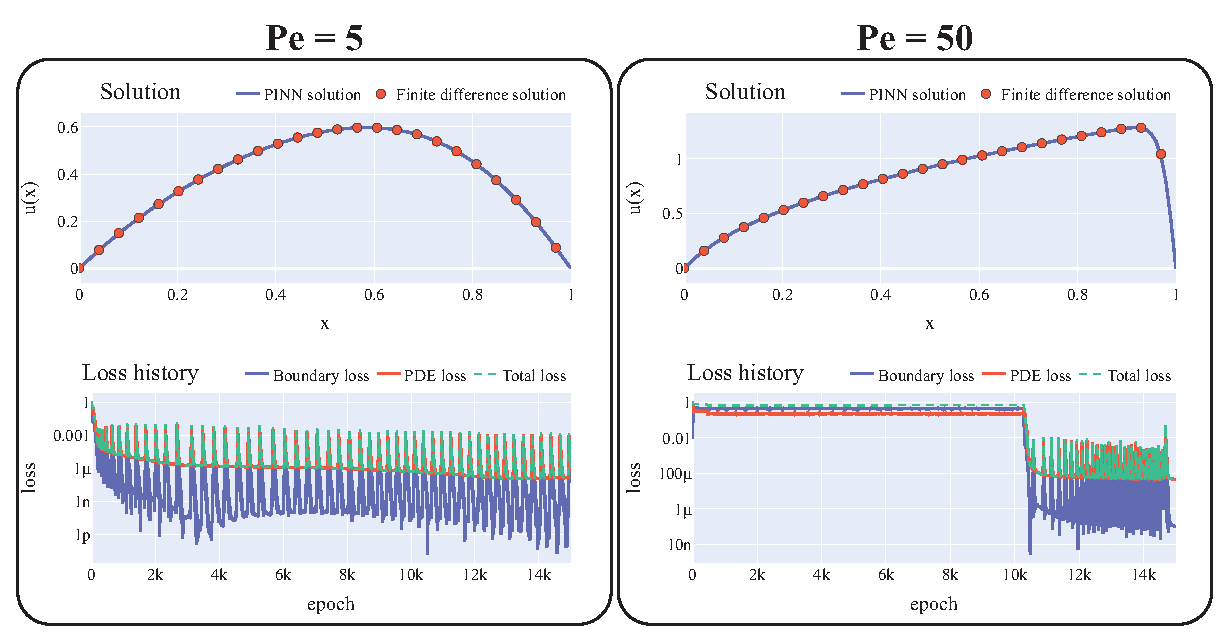
\includegraphics[width=1.0\textwidth]{images/stat_viscous_burgers.eps}
\caption{\label{fig:stat_viscous_burgers_results}PINN results (solution and loss histories) for the 1D stationary viscous Burgers equation shown for a case with (left) \(Pe = 5\) and (right) \(Pe = 50\). The PINN solutions are depicted by solid, blue lines while scatter points represent reference finite-difference solutions.}
\end{figure}

\subsubsection{\(Pe = 5\)}
\label{sec:org5dc6172}
We begin by investigating the capability of our PINN to solve
\cref{eqn:stationary_burgers} for \(Pe = 5\). Here, we expect
non-linearities to be not too significant, and hence our network should behave
similar to \cref{sec:poisson} and
\cref{sec:helmholtz}. Upon training our PINN with \(N_\pde = 100 , N_b = 2\) we
see the expected behavior and recover solutions
shown in the left column of \cref{fig:stat_viscous_burgers_results}, along with its loss
histories. We see that our PINN solution agrees with the reference solution,
with \(e_h = 6.4 \times 10^{-4}\). The loss history is dominated by \(\mse_\pde\) and steadily decreases with increasing epochs.

\subsubsection{\(Pe = 50\)}
\label{sec:org6a6f34d}
Next, we investigate the case with \(Pe = 50\), where effects of
non-linearities are expected to be significant. Here we expect a relatively
smooth solution in the bulk of the domain, with a rapid adjustment to the boundary
condition at \(x = 1\). Upon training our PINN with \(N_\pde = 100 , N_b = 2\) we
see this expected behavior and recover solutions shown in the right column of
\cref{fig:stat_viscous_burgers_results}, along with its loss histories.
We see that our PINN solution agrees with the reference solution,
with an \(e_h = 4.2 \times 10^{-3}\), indicating our ability to capture
non-linearities. Regarding its training, the PINN barely learns till around 10k epochs,
as the loss is almost constant. Then, after this
critical epoch number, it discovers
the solution manifold and the loss rapidly decreases. Beyond this
point, the loss history is dominated by \(\mse_\pde\) and maintains a near-steady value. Such network behavior is unique to this case, and
more investigations are necessary to uncover the network dynamics before and
after the critical epoch.

\subsection{PINN solutions of viscous Burgers equation}
\label{sec:burgers}
\newcontent{
We then increase the complexity of PDE from our previous section on
stationary viscous Burgers \cref{eqn:stationary_burgers} by adding in a temporal
evolution term. This results in the time evolving, nonlinear viscous Burgers
equation whose solutions \(u : (y, t) \mapsto \mathbb{R},~y \in [0, 1],~t \in [0, 1]\),
are described by
\begin{equation}
\label{eqn:burgers}
\begin{aligned}
	 \pde[ u ] := \frac{\partial u}{\partial t} + \frac{1}{2}\frac{\partial \left(u^2\right)}{\partial y} - \frac{1}{Pe}\frac{\partial^2 u}{\partial y^2} = 0
\end{aligned}
\end{equation}
coupled with suitable boundary conditions and an additional initial condition. Similar to the stationary Burgers
equation, viscous Burgers equation is useful in modeling fluid-dynamics applications.
Additionally, it finds use in nonlinear acoustics and even traffic-flow
problems \cite{miroe2017}! Indeed, typical solution to \cref{eqn:burgers} form
\emph{shock waves} which are regions where the solution \emph{folds} over itself due to
non-linearities (such shocks are depicted in our results below). As a result
of such folding, the
solution changes behavior dramatically within a short span of space-time
which then makes the resolution of such shocks non-trivial. Here we challenge
our PINNs to reproduce the shock behavior characteristic of \cref{eqn:burgers}.
}

\newcontent{
We have already seen the ability of PINNs to capture non-linear
effects moderated by the Péclet number \(Pe\) for realistic
conditions in \cref{sec:stationary_burgers}, in the context of viscous Burgers
equation. There, the solution was driven by an external forcing \(f\). Here
however, this forcing is absent. The solution evolution is then purely driven
by time \(t\), whose effects we access by modifying the solution profile at
the initial time \(t = 0\) for Dirichlet boundary conditions
\[ u_b(0, t) = 0;\quad  u_b(1, t) = 0 \]
to enforces absence of velocities on the walls at \(y = 0, 1\).
To compare against our PINN solutions in these settings, we once again rely
on numerical solutions \({u}_h\) based on finite-differences.
}

\begin{figure}[htbp]
\centering
\includegraphics[width=1.0\textwidth]{images/burgers_panel.eps}
\caption{\label{fig:burgers_results}PINN results (solution and loss histories) for the viscous Burgers equation (varying with space--time) shown for different initial profiles that develop a (left) shock and (right) rarefaction waves. We first show the PINN solutions, followed by error plots (which we obtain by comparing to reference numerical solutions). Finally, loss histories are shown.}
\end{figure}

\subsubsection{Shock waves}
\label{sec:org997b945}
\newcontent{
We begin by investigating the capability of our PINN to capture non-linear shocks in
\cref{eqn:burgers}. To instigate these shocks, we
choose the following initial solution profile
\[ u(y, 0) = \sin{2 \pi y}\]
}
\newcontent{
We train our PINN with \(N_\pde = 10000\) sampled on a \(100 \times 100\) uniform
grid of space-time. We set \(N_b = 300\) sampled uniformly on
the three boundaries---two for enforcing the boundary condition, and one for
enforcing the initial condition---each having \(100\) points. We showcase
the results obtained
in the left column of \cref{fig:burgers_results}. First, we show the
solution generated by the PINN on the top row. Here we see the
characteristic nature of shocks, with the red and blue regions come together
and collapse at the middle of the domain \(y = 0.5\). Next, we show the spatial
distribution of the relative errors (as percentages) obtained upon
comparison with the numerical solution. As
seen from this plot, the maximum errors are bounded \(< 3\%\), and close to
the shock location. Averaging these errors across the domain, we obtain \(e = 6 \times 10^{-3}\).
This confirms PINN's ability to capture PDE solutions in spatio-temporal
problems. Next, we present the PINN loss histories
during training.
Here, the loss history is dominated by \(\mse_\pde\) which decreases with
increasing epochs. This loss reflects the localized PDE errors seen in the
center of our space-time domain.
}

\subsubsection{Rarefaction waves}
\label{sec:org6472f69}
\newcontent{
Next, we investigate the formation of non-linear rarefaction waves with our PINN in
\cref{eqn:burgers}. To setup these rarefaction waves, we choose the following
initial solution profile
\[ u(y, 0) = -\sin{2 \pi y}\]
}

\newcontent{
Once more, we train our PINN with \(N_\pde = 10000\) sampled on a \(100 \times 100\) uniform
grid of space-time. We set \(N_b = 300\) sampled uniformly on
the three boundaries---two for enforcing the boundary condition, and one for
enforcing the initial condition---each having \(100\) points. We showcase
the results obtained
in the right column of \cref{fig:burgers_results}. First, we show the
solution generated by the PINN on the top row. We see the
characteristic nature of rarefaction waves, where the red and blue regions
which are initially close, diverge away from each other and fan out
from the middle of the domain at \(y = 0.5\). We then show the spatial
distribution of the relative errors (as percentages) obtained upon
comparison with the numerical solution. Once again the maximum errors are
bounded \(< 5\%\), but this time they are concentrated close to
the domain boundaries. Averaging these errors across the domain, we obtain \(e = 4.8 \times 10^{-3}\).
This provides additional evidence that PINNs can viably capture non-linear
spatio-temporal PDE solutions. Next, we present the PINN loss histories
during training.
Here, the loss history is dominated by \(\mse_{b}\) which decreases with
increasing epochs. This loss reflects the localized errors seen near the
boundary of our space-time domain.
}

\subsection{PINN solutions of 2D Laplace equation}
\label{sec:laplace}
\newcontent{
Finally we utilize the machinery of \cref{eqn:burgers} to demonstrate solutions
of the Laplace equation in fully two-dimensional settings. The solutions \(u : \gv{x} := (x, y) \mapsto \mathbb{R},~\gv{x} \in \mathcal{D}\) for some domain \(\mathcal{D}\)
are described by
\begin{equation}
\label{eqn:laplace}
\begin{aligned}
	\pde[ u ] &:= \nabla^2 u = 0 \\
	   		  &:= \frac{\partial^2 u}{\partial x^2} + \frac{\partial^2 u}{\partial y^2} = 0
\end{aligned}
\end{equation}
coupled with suitable boundary conditions. The Laplace equation is a special
case of the Poisson equation (see \cref{sec:poisson}) with \(f(\gv{x}) = 0\),
and hence has similar applications.
}

\newcontent{
While we have demonstrated the ability of PINNs to capture this PDE in
\cref{sec:poisson}, there we were limited to a rectangular domain in one-dimension.
Here we crucially extend it to higher-dimensions (2D) in complex geometries
of interest in design and engineering scenarios. In these settings, the
boundary conditions can be spatially varying and hence the
resulting solution is more challenging to capture.
}

\begin{figure}[htbp]
\centering
\includegraphics[width=1.0\textwidth]{images/laplace_panel.eps}
\caption{\label{fig:laplace_results}PINN results (solution and loss histories) for the 2D Laplace equation shown for a case in a (left) rectangular domain and (right) starfish domain. We first show the PINN solutions, followed by error plots (which we obtain by comparing to reference numerical solutions). Finally, loss histories are shown.}
\end{figure}

\subsubsection{Rectangular domain}
\label{sec:orgabbae02}
\newcontent{
We begin by testing our PINN architecture to solve \cref{eqn:laplace} in a
rectangular domain. Here we fix Dirichlet boundary condition in the
\(x\)-direction:
\[ u_b(0, y) = 0;\quad  u_b(1,  y) = 0\]
while in the \(y\)-direction we have a mixed boundary
condition, similar to \cref{sec:poisson}:
\[ u_b(x, 0) = 0 ;\quad \frac{\partial u_b}{\partial x}(x, 1) = \pi\left(
	\exp{\left(\pi\right)} + \exp{\left(-\pi\right)} \right) \sin\left( \pi x\right)\]
This case lends itself to a straightforward analytical solution:
\[
	\hat{u}(x, y) = \left(\exp{\left(\pi y\right)} - \exp{\left(-\pi y\right)} \right) \sin\left( \pi x\right)
	\]
}
\newcontent{
We train our PINN with \(N_\pde = 10000\) sampled on a \(100 \times 100\) uniform
grid with in the domain. We set \(N_b = 400\) once again sampled uniformly on
the four boundaries having \(100\) points each. We showcase the results obtained
in the left column of \cref{fig:laplace_results}. Here we first show the
solution generated by the PINN on the first row. Next, we show the spatial
distribution of the relative errors (as percentages) obtained upon
comparison with the analytical solution. As
seen from this plot, the maximum errors are bounded \(< 1\%\), and close to
the domain bottom boundaries. Averaging across the domain, we have error \(e = 5.2 \times 10^{-3}\).
This confirms PINN's ability to capture PDE
solutions in higher dimensional domains. Next, we present the PINN loss histories
during training.
Here, the loss history is constrained by both \(\mse_\pde\) and \(\mse_{b}\) and decreases slowly with increasing epochs. Both this
loss history and the concentration of PDE errors close to the bottom boundaries
indicate that the PINN has difficulty adjusting to the boundary condition.
Nevertheless, it is successfully able to propagate the boundary information
into the domain and capture the interior solutions.
}

\subsubsection{Starfish domain}
\label{sec:orgaed67f3}
\newcontent{
Finally, we challenge our PINN approach to capture solutions in complex
domains. Here we choose a domain resembling the shape of a starfish, shown
in the right column of \cref{fig:poisson_results},
characterized by the following function
\[ r = a \left( 1 + \epsilon \cos{\left( n \theta \right)} \right) \]
where
\[ r := \sqrt{x^2 + y^2} \; \quad \theta := \arctan{\left(y/x\right)} \]
are coordinates in the polar domain, \(a = 1, \epsilon = 0.4 , n = 5\). Here
\(r \in [0, r_o]\) and \(\theta \in [0, 2\pi]\), with \(r_o\)
representing the outer domain edge. In this complex shape setting, we
choose the following boundary condition,
\[ u_b(r_o, \theta) = \sin{\theta}\]
chosen for its simplicity while retaining (physical) periodicity around the curve.
Even with this simple parameterization, we do not have
analytical solutions, so we turn
to numerical solutions using an integral equations approach.
}

\newcontent{
Here, we train our PINN with \(N_\pde = 2500\), with a uniform
distribution of \(25\) points in the \(r\) domain and \(100\) points in
the \(\theta\) domain. We set \(N_b = 100\) sampled on the outermost
edge of the domain (shown as blue crosses in the middle row of the figure).
We recover the solutions shown in the right column of
\cref{fig:laplace_results}. Here we once again show the
solution generated by the PINN on the first row. Next, we show the spatial
distribution of the relative errors (as percentages) obtained upon
comparison with the analytical solution. As
seen from this plot, the maximum errors are bounded \(< 3\%\), and close to
the sharp(er) corners of the domain. Averaging across the domain, we have error \(e = 3.5 \times 10^{-2}\).
This re-confirms PINN's ability to capture PDE
solutions in complex, higher dimensional domains. Next, we present the PINN loss histories
during training.
Here, the loss history is constrained by boundary losses \(\mse_{b}\)
which decreases with increasing epochs. This once again indicates that the
PINN has difficulty adjusting to the boundary condition. As a final remark,
we note that we can potentially rectify the high boundary losses encountered in both cases
shown in this section by penalizing boundary losses more than the PDE loss
by setting \(\lambda_{\pde} < 1\).
}

\newcontent{
Finally, we demonstrate the versatility and robustness of PINNs by solving
PDEs on more complex shapes with varying boundary conditions, for a case
which is otherwise tedious to solve using conventional numerical algorithms.
We chose to parametrize the shape \emph{CS498DL} (chosen for its
relevance to the course) and solve the Laplace equation inside the
alphanumerical characters. We showcase this solution in
\cref{fig:cs498_poisson_results}. We remark that despite the complexity of this
problem we obtain solutions using the same machinery we built up thus far in a
straightforward manner, without the need for complicated, explicit treatment
at the domain boundaries.
}

\begin{figure}[htbp]
\centering
\includegraphics[width=1.0\textwidth]{images/CS498DL_cropped.eps}
\caption{\label{fig:cs498_poisson_results}Solution of a Poisson equation generated by PINNs within the shape \emph{CS498DL}. Each alphanumerical character is prescribed with a unique boundary condition resulting in varied, rich solutions seen in the interior.}
\end{figure}

\section{Conclusions}
\label{sec:org9701e2b}
\newcontent{
In summary, we successfully implemented and investigated PINN for solving
non-linear partial differential equations. We demonstrated PINNs’ ability to
solve equations of increasing complexity, from linear, 1D problems to
nonlinear, 2D problems. In particular, we first demonstrated PINN's utility in
solving 1D linear BVPs (Poisson, Helmholtz) with varying boundary conditions
and forcing functions, followed by a non-linear BVP (steady viscous Burgers).
We then extend this machinery to solve a more complex spatio-temporal
non-linear PDE in quasi-2D regime (unsteady viscous Burgers) where we showed
that PINNs could successfully capture the expected, non-trivial, non-linear
behaviors (shocks and rarefaction waves). We then demonstrated PINN solutions
on fully 2D BVPs (Laplace) on regular (rectangular) and arbitrary (starfish)
domains. Finally, we conclude
by presenting the versatility and robustness of PINN by solving a PDE
(Laplace) on a complex CS498 shape and varying boundary conditions, which is
otherwise difficult to solve by conventional numerical algorithms.
}
\section{Personal interests}
\label{sec:orgad03acb}
In our first project checkpoint we were asked to ``\emph{provide more information on}
\emph{how this topic relates to your backgrounds and any research projects outside}
\emph{of this class}''. This section intends to answer this question.

All team members are currently pursuing doctoral studies in continuum fluid
and solid mechanics using predominantly computational techniques. These involve
developing algorithms, implementing scalable software and using these to
investigate physics for rationally designing new applications. As part of this
process, we need to numerically solve multiple coupled PDEs, similar to those
demonstrated in this report, for large systems (containing \(10^7-10^{10}\)
degrees of freedom). In this context, we are interested in leveraging ML techniques to either
\begin{itemize}
\item rapidly find solutions to such large DOF PDEs
\item accelerate present numerical PDE solvers for improved speed
\item provide data-driven model closures when the PDE is unknown (such as in
turbulence)
\item provide black-box control capabilities in devising physics-based applications
\end{itemize}

\section{Contributions}
\label{sec:org3be66b6}
All three members were involved in project conceptualization, implementing the
software, running numerical experiments, analyzing and visualizing data and finally
preparing the report.


 \newpage

\bibliography{CS498DL_project}

\bibliographystyle{unsrt}
\end{document}
